
%(BEGIN_QUESTION)
% Copyright 2011, Tony R. Kuphaldt, released under the Creative Commons Attribution License (v 1.0)
% This means you may do almost anything with this work of mine, so long as you give me proper credit

Read selected portions of the Siemens ``SIMATIC S7-200 Programmable Controller System Manual'' (document A5E00307987-04, August 2008) and answer the following questions:

\vskip 10pt

Identify the different types of SIMATIC {\it timer} instructions, explaining how each one functions.

\vskip 10pt

Identify a practical application for a timer instruction programmed into a PLC.

\vskip 10pt

How long can one of these timer instructions time up to?  Based on this maximum value, how many bits do you think are used in the register to store a timer instruction's current value?

\vskip 10pt

What is meant by the {\it resolution} of a timer instruction?  How many different options do the SIMATIC instructions provide for resolution?

\vskip 10pt

Comment on how a SIMATIC timer's value is updated in a PLC program if the resolution is 1 ms, if it is 10 ms, and if it is 100 ms.  The Siemens S7-200 PLC handles each one differently!

\vskip 10pt

Sketch a simple ladder-diagram program for a Siemens S7-200 PLC whereby a switch connected to input {\tt I0.3} causes a timer to increment (count {\it up}) and then turn on an alarm light output {\tt Q0.9} after 5 seconds.  

\vskip 20pt \vbox{\hrule \hbox{\strut \vrule{} {\bf Suggestions for Socratic discussion} \vrule} \hrule}

\begin{itemize}
\item{} If you have access to your own PLC for experimentation, I urge you to write a simple {\it demonstration} program in your PLC allowing you to explore the behavior of these PLC instructions.  The program doesn't have to do anything useful, but merely demonstrate what each instruction does.  First, read the appropriate section in your PLC's manual or instruction reference to identify the proper syntax for that instruction (e.g. which types of data it uses, what address ranges are appropriate), then write the simplest program you can think of to demonstrate that function in isolation.  Download this program to your PLC, then run it and observe how it functions ``live'' by noting the color highlighting in your editing program's display and/or the numerical values manipulated by each instruction.  After ``playing'' with your demonstration program and observing its behavior, write comments for each rung of your program explaining in your own words what each instruction does.
\item{} Why do you suppose Siemens designed their timer instructions to update their current values differently, depending on the programmed resolution of the timer?  Why not make all timer instructions update similarly, regardless of resolution?
\end{itemize}

\underbar{file i00229}
%(END_QUESTION)





%(BEGIN_ANSWER)


%(END_ANSWER)





%(BEGIN_NOTES)

The three SIMATIC timer instructions include the On-Delay Timer (TON), Retentive On-Delay Timer (TONR), and Off-Delay Timer (TOF).  Both the TON and TONR timer instructions count time when activated, the difference between them being what happens when their inputs are de-activated: the TON immediately clears while the TONR retains its count value.  The TOF timer instruction counts time when its input is de-activated.

SIMATIC timer instructions may be reset using a special Reset function, which looks like a coil instruction with the letter ``R'' inside of it (equivalent to Allen-Bradley's ``RES'' coil).

\vskip 10pt

These counters have a maximum count value of 32,767 (15 bit binary number), in resolutions of 1 ms, 10 ms, and 100 ms.  For example, a count value of 5000 with 1 ms resolution is 5000 milliseconds or 5 seconds.  The same count value with a 10 ms resolution is 50000 ms or 50 seconds.

\vskip 10pt

If the resolution of a timer is set for 1 ms, the timer's count value will be updated throughout the program scan (i.e. multiple times if the scan cycle time exceeds 1 ms).  This means a timer's current value can change at different points within a ladder program!  

If the resolution is set for 10 ms, the timer count updates at the beginning of the scan cycle, with the current value remaining constant throughout the duration of the scan.  

If the resolution is set for 100 ms, the timer count updates only when the timer instruction is reached in the program scan (page 198).

$$\includegraphics[width=15.5cm]{i00229x01.eps}$$

%INDEX% Reading assignment: Siemens S7-200 system manual (timer instructions)

%(END_NOTES)


